\documentclass[11pt,letterpaper]{article}

\usepackage[spanish,es-tabla,es-nodecimaldot]{babel}
\usepackage{amsmath}
\usepackage[utf8]{inputenc}
\usepackage[T1]{fontenc}
\usepackage{lmodern}
\usepackage{graphicx}
\usepackage{listings}
\usepackage{anysize} 
\usepackage{fancyhdr}
\usepackage{amsmath}
\usepackage{pdfpages}
\usepackage{graphics}
\usepackage{capt-of}
\usepackage{tabularx}
\usepackage{rotating}
\usepackage{tikz}
\usepackage[colorlinks=true,plainpages=true,citecolor=blue,linkcolor=blue]{hyperref}


\marginsize{2cm}{2cm}{2cm}{2cm}
\pagestyle{fancy}
\fancyhf{Sistemas celulares}
\fancyhead[L]{\footnotesize UPIITA-IPN} 
\fancyhead[R]{\footnotesize 2TV7} 
\fancyfoot[R]{\footnotesize Tarea 3}
\fancyfoot[C]{\thepage}
\fancyfoot[L]{\footnotesize } 

\renewcommand{\footrulewidth}{0.4pt}
\renewcommand{\spanishtablename}{Tabla}
\renewcommand{\labelitemii}{$\star$}
\graphicspath{ {C:/Users/Anselmo/Documents/GitHub/upiita-SistemasCelulares/Tarea3/imagenes} }

\begin{document}

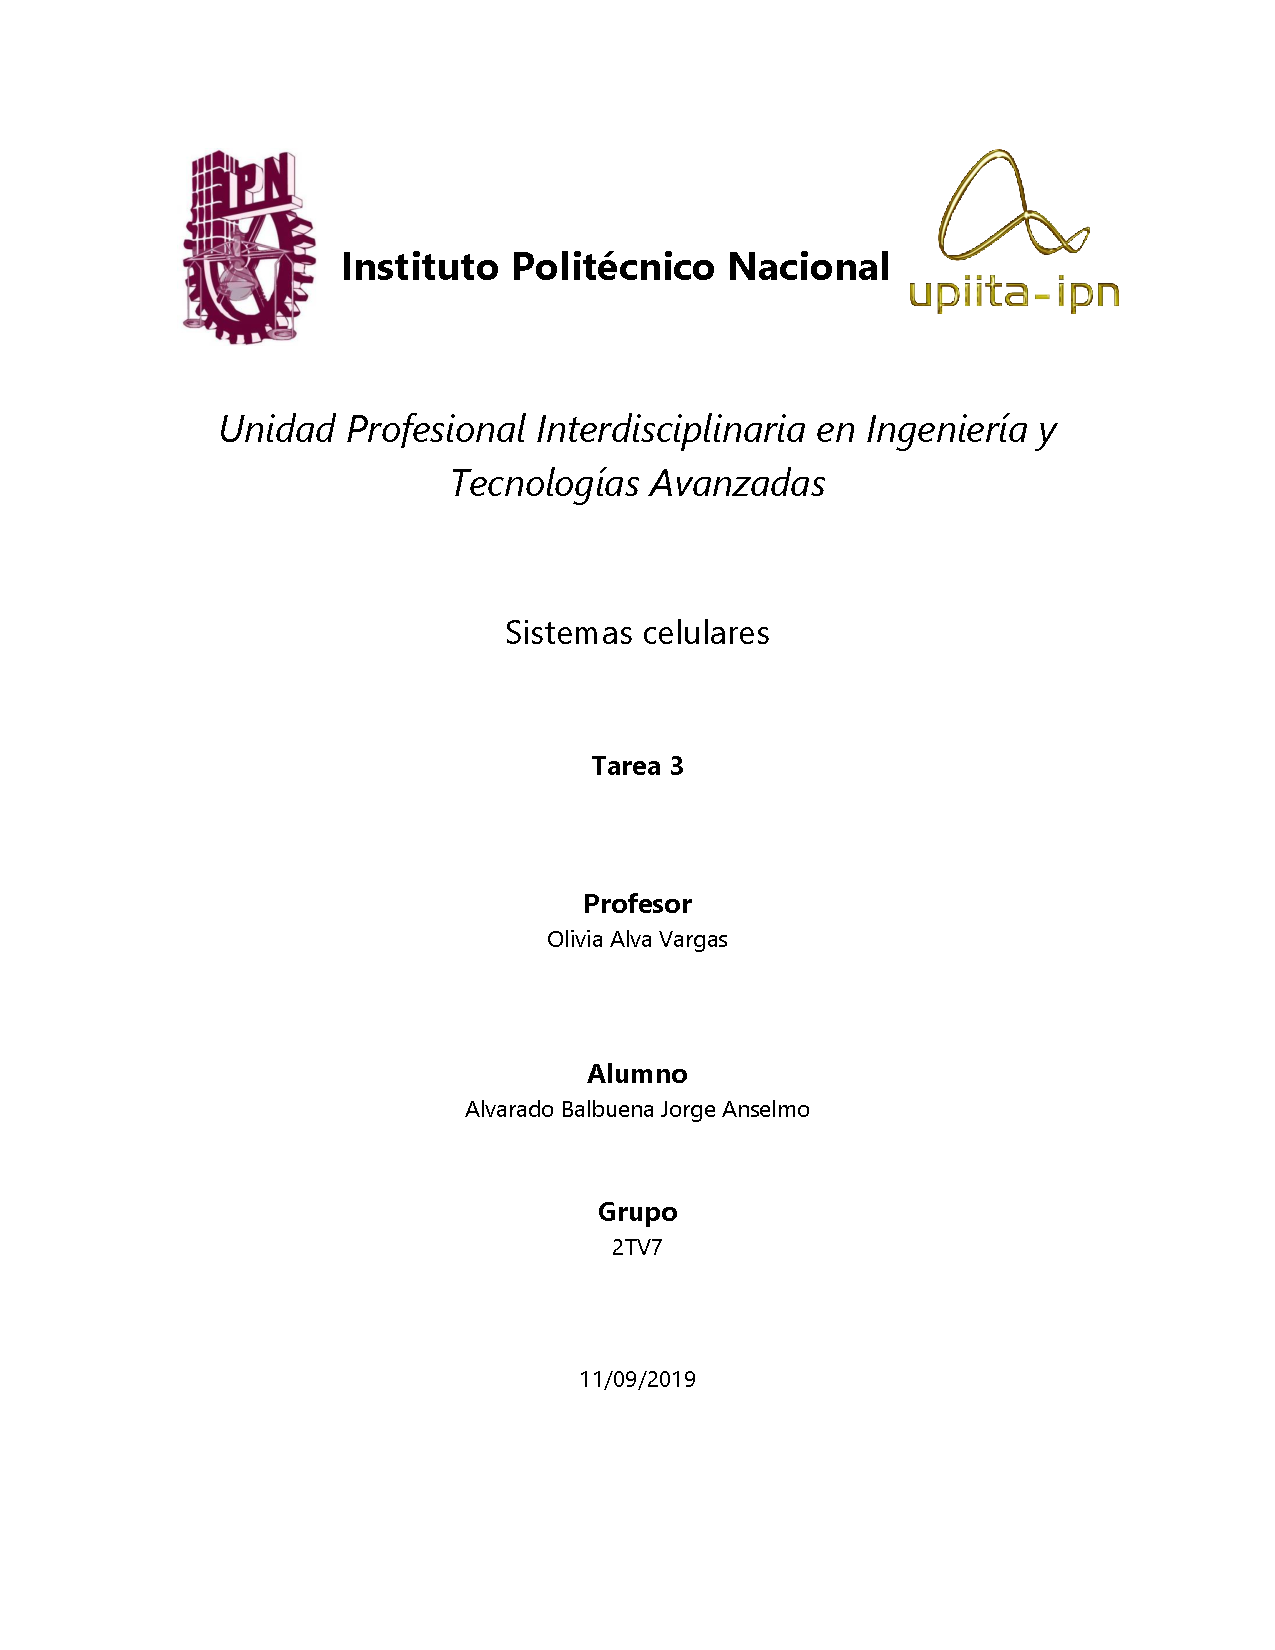
\includepdf[pages={1}]{Portada}

\newpage
\tableofcontents
\listoffigures
\listoftables

\newpage
\section{Antecedentes}
La población actual del municipio de Nezahualcóyotl es de 1,228,54 habitantes.
La población con la cual se realizó el estudio anterior corresponde al 5\% de 
la población actual. El resultante de esta operación es de 61,432 habitantes. 
\\ \\
Para el siguiente estudio se propone que el aumento de población de los 80s 
sea de un 1.6\%. Este supuesto se hace pensando en el cambio de AMPS a GSM ya 
que este aumento de población se le proporcionará servicio. El 1.6\% de la 
población de los 80s es 98,291.2. El total de población para el estudio actual 
es de 153,581 habitantes.
\\ \\
Las razones por las cuales se propone este aumento de población están en función 
del aumento promedio en la población y a la oferta de servicios que hacen que los 
habitantes opten por quedarse y continuar su vida dentro de la localidad. Algunos 
de estos servicios son el aumento de unidades académicas, la normalización de 
servicios de agua, servicios sanitarios y de entretenimiento. 
\\ \\
Otra razón de peso en el aumento de la población es la migración continua del 
interior de la república a una zona cerca de la Ciudad de México a un no tan alto 
costo de vivienda.
\\ \\
Los datos del estudio anterior con el sistema AMPS se enlistan a continuación.
\begin{itemize}
    \item CH: 2010.
    \item N: 49,618.2.
    \item A: 2480.91.
    \item $BW_{CH}:30KHz$.
    \item $BW_{SIS}:24MHZ$.
    \item Área: $63.74km^2$
\end{itemize}

\newpage
\section{Desarrollo}
\subsection{Fundamento}
Uno de los puntos a resaltar en el cambio de AMPS a GSM es el cambio del 
método de acceso de división de frecuencia por división de tiempo. Ahora todas 
las células del clúster trabajaran sobre la misma banda de frecuencias. Para 
obtener el numero de canales con este nuevo método, se parte de tres datos 
que fueron obtenidos en AMPS del estudio anterior, los canales de AMPS, los 
Erlang y el número de llamadas a proporcionar.
\\ \\
Este cambio de sistema ofrece un nuevo grado de servicio (GoS) igual a 99.8\%.

\begin{equation}
    \frac{100-99.8}{100}=0.002
\end{equation}
\\
Con el valor calculado y el número de canales obtenidos en el estudio anterior se puede 
obtener el numero de circuitos y los erlangs correspondientes a este nuevo resultado.

\begin{figure}[ht]
    \centering
    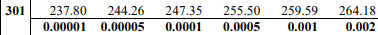
\includegraphics[width=0.8\textwidth]{imagenes/erl.png}
    \caption{Valor del GoS en la tabla de erlangs.}
\end{figure}


$n=301 => A=264.18 \ Erlnag$
\\ 
$n_c=2010->A_c=1764.12 \ Erlnag$
\\ \\
Posteriormente se calculará la nueva eficiencia espectral.
\begin{equation}
    \eta=\frac{Tráfico \ Erlang}{BW_{SIS}*Área}=\frac{1764.12}{24MHz*63.74km^2}=1.153 \ Erlnag/MHz/Km^2
\end{equation}
\\
Ahora el número de llamadas con la siguiente expresión resolviendo para $N$.
\begin{equation}
    A=\frac{N*\overline{t}}{hp}
\end{equation}
\begin{equation}
    N=\frac{A*hp}{\overline{t}}=\frac{1764.12*3600}{180}=35282.4 \ llamadas
\end{equation}
\\
Esta información deja una relacción de:
\begin{equation}
    N=\frac{N}{p(00s)}=\frac{35282.4}{98291.2}=0.358 \ llamadas \ por \ usuario
\end{equation}

\newpage
\subsection{Parámetros de Poisson}
Para obtener el numero de canales en TDMA se debe de multiplicar los canales 
en AMPS.

\begin{equation}
    nTDMA=CH_{AMPS} \ * \ 8=16080
\end{equation}

\begin{figure}[ht]
    \centering
    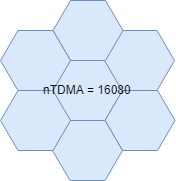
\includegraphics[width=0.3\textwidth]{imagenes/cluster.png}
    \caption{Total de canales en el clúster.}
\end{figure}

Posteriormente se puede calcular lambda con la siguiente expresión, que es la 
intensidad de tráfico. Se propone que hp sea 3600 segundos.
\begin{equation}
    \lambda=\frac{N}{hp}=\frac{35282.4}{3600}=9.8 \ \frac{N}{S}
\end{equation}
\\
Conociendo $\lambda$ se calcula el espacio de arribos con la siguiente expresión.
\begin{equation}
    \frac{1}{\lambda}=0.102
\end{equation}
\\
Retomando el tiempo promedio $\overline{t}$, también $t_m$, se obtiene la tasa de espera $\mu$ 
con la siguiente expresión. 

\begin{equation}
    \mu=\frac{1}{\overline{t}}=\frac{1}{180}=5.55\overline{5} \ ms
\end{equation}
Por ultimo se calcula la espera media de ocupaciones demoradas $t_w$ y el tiempo máximo 
de espera $\overline{t}_w$
\begin{equation}
    t_w=\frac{t}{t_m}=\frac{5}{180}=0.02\overline{7} seg
\end{equation}
\begin{equation}
    \overline{t}_w=t_w*P(>0)=t_w*\lambda=t_w*\frac{N}{hp}=0.02\overline{7}*\frac{35282.4}{3600}=0.272seg
\end{equation}


\newpage
Los datos obtenidos anteriormente servirán para calcular los parámetros que entrega 
la distribución de Poisson. En seguida se muestra un diagrama con los parámetros que se 
obtendrán.

\begin{figure}[ht]
    \centering
    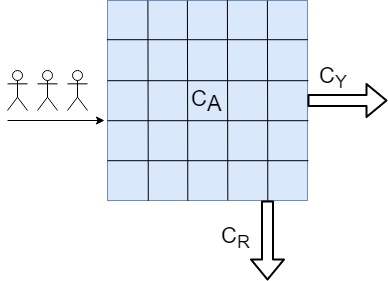
\includegraphics[width=0.7\textwidth]{imagenes/pos.png}
    \caption{Parámetros que entrega la distribución de Poisson.}
\end{figure}

Primero se calcula las gestionadas atendidas $C_{A}$ con la siguiente expresión.
\begin{equation}
    C_A=n_{TDMA} \ * \ \lambda = 16080 * 9.8= 157,549.75
\end{equation}

Ahora las llamadas cursadas $C_Y$ con un Erlang B igual a 0.01.
\begin{equation}
    C_Y=C_A(1-B)=157,549.75(1-0.01)=156,018.772
\end{equation}

Por ultimo las llamadas rechazadas.
\begin{equation}
    C_R=C_A*B=157,549.75*0.01=1,575.497
\end{equation}

Con la información anterior se puede obtener las gestiones efectivas.
\begin{equation}
    C_A-C_R=157,549.75-1,575.497=155,974.253
\end{equation}

\newpage
En la siguiente tabla se concentran los resultados obtenidos en este estudio.
\begin{table}[ht]
    \centering
    \begin{tabular}{|c|c|}
    \hline
    Parámetro & Valor   \\ \hline
    Erlang A & $1764.12$  \\ \hline
    Erlang B & $0.01$  \\ \hline
    $\eta$ & $1.153 \ Erlnag/MHz/Km^2$  \\ \hline
    N & $35282.4 \ llamadas$  \\ \hline
    hp & $3600 \ seg$  \\ \hline
    $\overline{t}$ o $t_w$ & $180 \ seg$  \\ \hline
    nTDMA & $16080$ canales  \\ \hline
    $\lambda$ & $9.8 \ \frac{N}{s}$  \\ \hline
    $\frac{1}{\lambda}$ & $0.102$  \\ \hline
    $\mu$ & $5.55$ ms  \\ \hline
    $t_m$ & $0.027$ seg  \\ \hline
    $t_w$ & $180$ seg \\ \hline
    $\overline{t}_w$ & $0.272$ seg  \\ \hline
    $C_A$ & $157,549.75$  \\ \hline
    $C_Y$ & $156,018.772$  \\ \hline
    $C_R$ & $1,575.497$  \\ \hline
    Gestiones efectivas & $155,974.253$  \\ \hline
    \end{tabular}
    \caption{Tabla de resultados.}
    \label{tab:my-table}
\end{table}

\newpage
\section{Conclusión}
La población estimada para la realización de este estudio y la cual se tiene registrada 
en los inicios de la década de los 2000s varia bastante. En seguida se muestra una 
tabla mostrando la evolución demográfica del municipio.
\begin{figure}[ht]
    \centering
    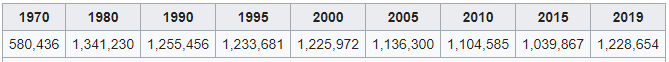
\includegraphics[width=0.9\textwidth]{imagenes/demo.png}
    \caption{Evolución demográfica del municipio de Nezahualcóyotl.}
\end{figure}

Para estos datos el cambio de AMPS a GSM resulta en que el servicio se clasificaría como 
insuficiente. Aunque hay factores demográficos y socioeconómicos que hay que temar en 
cuenta. El primero de ellos, es considerado como uno de los municipios con mayor densidad 
poblacional. Así que si se pusiera en uso el sistema GSM en horarios de noche-madrugada-mañana, 
el sistema dejaría sin servicio a un gran número de la población. 
\\ \\
Pero ¿por qué se menciona 
en concreto este horario? Como gran parte de los municipios del Estado de México que se 
encuentra alrededor de la Ciudad de México, también llamada zonza conurbada, es considerada 
una ciudad dormitorio por su carácter mayoritariamente residencial. Esto quiere decir que 
la mayor parte de la población económicamente activa trabaja en otra zona, para en este caso 
particular, la Ciudad de México. Otra razón por la cual mencionar este horario, es que la 
población económicamente activa mayor a 30 años del municipio es de aproximadamente un 85.21\%. 
\\ \\
De este porcentaje el 70,77\% son hombres y 39,52\% son mujeres. Por lo que la noche, cuando 
un gran número de población regresa, la madrugada, cuando la mayor parte de la población se 
encuentra en la zona y la mañana, cuando esa población que regreso vuelve a salir, son los 
periodos en lo que el sistema tiene una mayor demanda. Por lo que esto deja al día corriente 
como el horario cuando mejor servicio podría proporcionarse a la población. Se tiene que 
señalar que en caso de el suceso de una situación extraordinaria el sistema podría presentar 
deficiencias dejando a un gran numero de usuario sin servicio, aun tomando en consideración 
el reinicio del uso de los circuitos cada hora.
\end{document}